\documentclass[12pt,a4paper]{scrartcl}
\usepackage[utf8]{inputenc}
\usepackage{graphicx}
\usepackage{ngerman}
\usepackage{url}
\usepackage{amsmath}
\usepackage{caption}
\usepackage{wrapfig}
\usepackage{eurosym}
\usepackage{biblatex}
\usepackage{url}
\usepackage{color}
\usepackage{listings}
\usepackage{hyperref}
\usepackage[table]{xcolor}
\linespread{1.4}

\definecolor{mygreen}{rgb}{0,0.6,0}
\definecolor{mygray}{rgb}{0.5,0.5,0.5}
\definecolor{mylightgray}{rgb}{0.7,0.7,0.7}
\definecolor{mylightergray}{rgb}{0.9,0.9,0.9}
\definecolor{mymauve}{rgb}{0.58,0,0.82}

\let\origitemize\itemize
\def\itemize{\origitemize\itemsep0pt}

\lstset{ 
  backgroundcolor=\color{white},   
  basicstyle=\ttfamily\footnotesize,          
  breakatwhitespace=false,         
  breaklines=true,  
  commentstyle=\color{mygreen}, 
  escapeinside={\%*}{*)}, 
  extendedchars=true,             
  keepspaces=true,                 
  keywordstyle=\color{blue},
  language=Octave,
  numbers=left,                   
  numbersep=15pt,                  
  numberstyle=\tiny\color{mygray}, 
  showspaces=false,                
  showstringspaces=false,          
  showtabs=false,                  
  stringstyle=\color{mymauve},
  tabsize=2,
  title=\lstname,
  captionpos=b
}

\renewcommand*\lstlistingname{Codebeispiel}    %Rename Listings

\renewcommand*\thesection{\arabic{section}}

\makeatletter
\renewcommand\subparagraph{\@startsection{subparagraph}{5}{\parindent}%
    {3.25ex \@plus1ex \@minus .2ex}%
    {0.75ex plus 0.1ex}% space after heading
    {\normalfont\normalsize\bfseries}}
\makeatother

\begin{document}
\title{Praktikum Data Mining}
\subtitle{Energieverbrauch und CO2-Emmisionen \newline Vorhersage und Clustering auf Finanzdaten}
\author{Oliver Fesseler \and Maria Florus\ss \and Stefan Seibert \and  Daniel Grie\ss haber}
\maketitle
\newpage
\tableofcontents
\newpage

\part*{Energieverbrauch und CO\textsubscript{2}-Emmission}

\section*{Datenverwaltung und Statistik}
\subsection*{Einlesen der Daten, Hinzuf\"ugen der GPS Koordinaten, Abspeichern in neuer Datei}
Bei der Umsetzung der Aufgaben haben wir mit verschiedenen Darstellungsformen der Daten experimentiert. Im ersten Plot fallen vor allem die Vielverbraucher einzelner Energieformen auf. Beim zweiten Plot k\"onnen die verschiedenen Energiemixe pro Land direkt miteinander verglichen werden, da sie alle im selben Ma\ss stab nebeneinander dargestellt werden.

\subparagraph{ Ausgehend von der implementierten Visualisierung des Energieverbrauchs der L\"ander: Nennen Sie die 3 Ihrer Meinung nach interessantesten Beobachtungen.}

\begin{enumerate}
\item Durch die wenigen Industriel\"ander mit signifikant h\"oherem Energieverbrauch, wie China oder die USA, wird der Plot so verzerrt, dass die L\"ander mit durchschnittlichem Verbrauch im Plot so gestaucht werden, dass sie kaum zu erkennen sind. Dies k\"onnte behoben werden, wenn die Daten mit den Einwohnerzahlen aller L\"ander normalisiert werden w\"urden. So k\"onnte der Pro-Kopf-Verbrauch berechnet werden, was einen besseren Vergleich der einzelnen L\"ander bietet.
\item Dieses Prinzip wird klar bei der Betrachtung von China und Indien, die von der Einwohnerzahl her vergleichbar sind (China 1,3 Mrd., Indien 1,2 Mrd.\footnote{Stand 2012, Quelle: Wikipedia}). China zeigt einen weitaus h\"oheren Verbrauch als Indien an den in beiden L\"andern h\"aufigen Energieformen Kohle und \"Ol.
Zus\"atzlich w\"aren noch andere Normalisierungsfaktoren interessant:
\begin{itemize}
\item Bruttoinlandsprodukt
\item Au\ss enhandelsstatistik oder Export der L\"ander in US\$
\item Technologieindex
\end{itemize}
\item Die zwei L\"ander mit dem h\"ochsten Energieverbrauch sind China und die USA. Dies f\"allt bei der Betrachtung des Gesamtenenergieverbrauchs auf. Bei der Betrachtung des Verbrauchs einzelner Energieformen wirkt es als sei China durch seinen hohen Kohleverbrauch weit vor den USA.
\end{enumerate}

\subparagraph{Abgabe: Relevante Dateien}
\begin{itemize}
\item \lstinline{energy_consumption_per_country.py} und \lstinline{energy_consumption_per_country_V2.py} \\- Implementierung Aufgabe 2.1.2: 1) - 2)
\item \lstinline{energy_consumption_per_country.pdf} \\- Ausgabe des Skripts \lstinline{energy_consumption_per_country.py} 
\item \lstinline{energy_consumption_per_country_V2.pdf} \\- Ausgabe des Skripts \lstinline{energy_consumption_per_country_V2.py}
\item \lstinline{appendGeoCoordinates.py} \\- Implementierung Aufgabe 2.1.2: 3) - 5)
\item \lstinline|EnergyMixGeo.csv|  \\- Ausgabe des Skripts \lstinline{appendGeoCoordinates.py}
\end{itemize}





\subsection*{Statistik der Daten}

\subparagraph{Erkl\"aren Sie s\"amtliche Elemente eines Boxplot (allgemein). }
\begin{figure}[!h]
\centering
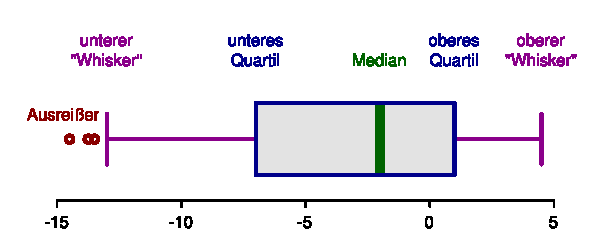
\includegraphics[width=0.7\textwidth]{Plots/Elements_of_a_boxplot.pdf}
\end{figure}
\begin{itemize}
\item Ausrei\ss er (\grqq Outliers\grqq ), in Python mit 'sym' zu setzen. \\
Daten die au\ss erhalb der Whisker liegen und somit als Ausrei\ss er deklariert werden.
\item Whisker, L\"ange in Python mit 'whis' zu setzen.\\
Standartm\"a\ss ig die 1,5-fache L\"ange des entsprechenden Quartils. 
\item Quartil\\
Die Quartile sind Bestandteile der Box, welche 50 \% aller Daten enth\"alt. Dabei enth\"alt das obere Quartil, die 25\%, die \"uber dem Median, das untere Quartil, die 25\%, die unter dem Median liegen.
\item Median\\
Der mittlere Wert (nicht Mittelwert oder Durchschnitt), der aus dem gesamten Datensatz ermittelt wird. Er teilt den Boxplot in zwei H\"alften, die wiederum jeweils in Whisker und Quartil unterteilt werden.
\end{itemize}

\subparagraph{Diskutieren Sie die im Boxplot angezeigte Statistik der Energieverbrauchdaten.}
\begin{itemize}
\item Durch den signifikant h\"oheren Verbrauch von China und den USA wird beim Anzeigen der Ausrei\ss er der restliche Boxplot soweit gestaucht, dass vern\"unftigen Daten mehr abgelesen werden k\"onnen. 
Um die Verteilung innerhalb der verschiedenen Boxplots besser vergleichen zu k\"onnen, entschlossen wir uns au\ss erdem jede Energieform in einem einzelnen Subplot darzustellen. 
\item Im Gesamtplot lassen sich die einzelnen Energieformen gut miteinander vergleichen, in den einzelnen Plots k\"onnen die Verteilungen innerhalb der Plots besser dargestellt werden.  
\item Beim Boxplot der nuklearen Energieform f\"allt auf, dass der Median samt unterem Quartil und unterem Whisker auf 0 liegt. Dies liegt daran, dass weniger als die H\"alfte aller L\"ander nukleare Energie verwenden. 
\item Im Gesamtplot kann man erkennen, dass \"Ol die einzige Energieform ist, deren unterer Whisker nicht auf 0 liegt. Also verwendet jedes in Betracht gezogene Land \"Ol. Jede andere Energieform wird von mindestens einem Land nicht verwendet. 
\end{itemize}

\subparagraph{Abgabe: Relevante Dateien}
\begin{itemize}
\item \lstinline{enegryStatistics.py} \\- Implementierung Aufgabe 2.1.3: 1) - 3)
\item \lstinline{energyconsumption_by_energyform_in_seperate_subboxplots.pdf} und \\ \lstinline{energyconsumption_by_energyform_in_one_plot.pdf} \\- Ausgabe des Skripts \lstinline{enegryStatistics.py}
\end{itemize}


\section*{Anwendung von Verfahren des un\"uberwachten Lernens auf Energieverbrauchsdaten}

\subsection*{Hierarchisches Clustering}
\subparagraph{Was wird beim Standardisieren gemacht? Welcher Effekt k\"onnte ohne Standardisieren beim Clustering eintreten (insbesondere wenn die euklidische Metrik verwendet wird)?}
Ohne Standardisieren ist die \"Ahnlichkeit des Gesamtverbrauchs ausschlaggebender als die \"Ahnlichkeit des Energiemixes. So werden eher L\"ander mit niedrigem Gesamtverbrauch gruppiert, als sie anhand ihres Energiemixes zu clustern. Dies kommt daher, dass die euklidische Metrik die geometrische Distanz zwischen zwei Punkten im Mehrdimensionalen Raum ber\"ucksichtigt. Zeigen zwei Vektoren in dieselbe Richtung, sind sich demnach vom Energiemix sehr \"ahnlich, haben aber unterschiedliche L\"angen, also einen unterschiedlich hohen Energieverbrauch, dann haben sie auch eine hohe euklidische Distanz und werden nicht demselben Cluster zugeordnet.
Durch das Standardisieren werden die L\"angen der Vektoren normiert und so ein Vergleich erst m\"oglich.

\subparagraph{Erk\"aren Sie die beim hierarchischen Clustering einstellbaren Parameter \lstinline{linkage-method} und \lstinline{metric}. Welche Metrik ist Ihrer Meinung nach f\"ur diese Anwendung geeignet? Warum?}

\"Uber die \lstinline{linkage-method} wird festgelegt, wie die Cluster hierarchisch angeordnet werden. Dabei kann zwischen verschiedenen Methoden gew\"ahlt werden: Beispielsweise kann die mittlere (average), die kleinste (single) oder die gr\"o\ss te (complete) Distanz zweier Punkte aus beiden Clustern, oder die Distanz der beiden Clusterschwerpunkte (weighted), gemessen werden. 
Die \lstinline{metric}  bestimmt die \"Ahnlichkeit zwischen zwei Punkten. Hierbei kann zwischen verschiedenen Metriken gew\"ahlt werden, wobei in unserem Fall \"Ahnlichkeitsma\ss e f\"ur boolsche Werte vernachl\"assigt werden k\"onnen. 
Die \"Ahnlichkeit kann \"uber die euklidische Distanz gemessen werden, allerdings wird hier nur die geometrische Distanz gewertet und nicht die Richtung. Weiterhin kann Cosinus-Distanz angewandt werden, bei der die Richtung der Vektoren mehr ins Gewicht f\"allt als die L\"ange. 
Bei der Pearson-\"Ahnlichkeit wird zus\"atzlich die Durchschnittsl\"ange miteinbezogen und mit der tats\"achlichen L\"ange verrechnet. Dadurch erweist sich dieser Algorithmus als am besten geeignet. 


\subparagraph{Welches Land ist bez\"uglich des Verbrauchs der hier betrachteten Energiequellen Deutschland am \"ahnlichsten, wenn f\"ur die linkage-method \lstinline{average} und die Metrik \lstinline{correlation} konfiguriert wird?}
\textbf{Antwort:} Belgien

\subparagraph{Charakterisieren Sie die 4 Cluster. Was ist typisch f\"ur die jeweiligen Cluster?}
\begin{itemize}
\item Cluster 0 ist einigerma\ss en gleichverteilt, wobei Wasserkraft den geringsten Anteil ausmacht. Im Vergleich zu den anderen Clustern ist der Anteil an aus Atomkraft gewonnener Energie sehr hoch. 
\item Cluster 1 zeichnet einen gro\ss en Verbrauch an fossilen Brennstoffen aus.
\item Cluster 2 ist das kleinste Cluster und unterscheidet sich vor allem durch seinen hohen Kohleverbrauch von den anderen Clustern.
\item Cluster 3 verzeichnet im Gegensatz zu allen anderen Clustern einen relativ hohen Wasserkraftanteil. 
\end{itemize}

Fasst man den gesamten Energieverbrauch jedes jeweiligen Clusters zusammen\\ (\lstinline{individual_clusters_total.pdf}), erkennt man, dass die Charakteristik des Gesamtverbrauchs eines Clusters sehr stark von einzelnen L\"andern abh\"angt. So diktieren China und die USA den Gesamtverbrauch in ihrem Cluster. Gleichzeitig zeigt sich allerdings auch die Tendenz des gesamten Clusters. 

\subparagraph{Abgabe: Relevante Dateien}
\begin{itemize}
\item \lstinline{energyClustering.py} \\- Implementierung Aufgabe 2.2.1: 1) - 5)
\item \lstinline{dendrogram.pdf}, \lstinline{individual_clusters.pdf} und \lstinline{individual_clusters_total.pdf}\\- Ausgabe des Skripts \lstinline{energyClustering.py}
\end{itemize}

\subsection*{Dimensionalit\"atsreduktion}

\subparagraph*{Welches Land ist nach dieser Darstellung Deutschland am \"ahnlichsten?}
\textbf{Antwort:} S\"udkorea
\subparagraph*{Warum entspricht die hier dargestellte \"Ahnlichkeit nicht der im oben erzeugten Dendrogram?}
\begin{enumerate}
\item Da wir die Darstellung selbst optisch interpretiert und die Distanz zwischen den Punkten als \"Ahnlichkeitsma\ss verwendet haben, haben wir die \"Ahnlichkeit nach der euklidischen Metrik bestimmt. 
\item Auch im Dendrogramm waren sich Deutschland und S\"udkorea relativ \"ahnlich. Durch die Reduktion der Dimensionen von f\"unf auf zwei gehen zwangsweise Informationen verloren. 
\end{enumerate}

\subparagraph{Abgabe: Relevante Dateien}
\begin{itemize}
\item \lstinline{energyReduceDim.py} - Implementierung Aufgabe 2.2.2: 1) - 3)
\item \lstinline{energyReduceDim_total.pdf}- Ausgabe des Skripts \lstinline{energyReduceDim.py}
\item \lstinline{energyReduceDim_section.pdf}- Ausschnitt aus \lstinline{energyReduceDim_total.pdf}
\end{itemize}

\section*{\"Uberwachtes Lernen: Sch\"atzung der CO\textsubscript{2}-Emmission}

\subsection*{Feature Selection}

\subparagraph{Welche 3 Merkmale haben den st\"arksten Einflu{\ss} auf das Ausgabemerkmal CO\textsubscript{2}-Emmission? Wie gro{\ss} sind die vom Programm ausgegebenen Scores?}
\begin{center}
\begin{tabular}{l r}
Kohle & 378.266881\\
\"Ol & 220.010151\\
Wasser & 79.045401\\
Gas & 46.002230\\
Nuklear & 34.572086
\end{tabular}
\end{center}

\subparagraph{Abgabe: Relevante Dateien}
\begin{itemize}
\item \lstinline{energyFeatureSelection.py} - Implementierung Aufgabe 2.3.1: 1) - 3)
\end{itemize}


\subsection*{Regression mit Epsilon-SVR}
\subparagraph{Optimieren Sie die SVR-Parameter C und Epsilon so dass der Score in der Kreuzvalidierung minimal
wird. Welche Werte f\"ur C und Epsilon liefern das beste Ergebnis?}

Die besten Ergebnisse erhielten wir f\"ur C = 0.01 und $\varepsilon$ = 0.001

\subparagraph{F\"ur das SVR-Objekt k\"onnen die Koeffzienten der linearen Abbildung, welche durch die trainierte
SVR realisiert wird, ausgegeben werden: \lstinline{meineSVR.coef\_}. Notieren Sie diese Koeffzienten f\"ur die
beste SVR.}

\begin{center}
\begin{tabular}{c c c c c}
\"Ol & Gas & Kohle & Nuklear & Hydro\\
$-3.0690410$ & $-2.3485549$ & $-3.9608432$ & $4.1970815e-04$ & $4.1138445e-04$
\end{tabular}
\end{center}
 
\subparagraph{Welchen Aufschluss geben diese Koeffzienten \"uber den Einfluss der einzelnen Eingangsmerkmale
auf das Ausgangsmerkmal?}

Die Koeffizienten geben an, wie sehr die entsprechende Energieform Einfluss auf die CO\textsubscript{2}-Emmission hat. \"Ol, Kohle und Gas haben demnach einen sehr viel gr\"o\ss eren Einfluss als Energie aus Atom- und Wasserkraft. 


\subparagraph{Wie gro{\ss} ist die mittlere absolute Differenz zwischen Soll- und Ist-Ausgabe f\"ur die beste SVR?
Diskutieren Sie dieses Ergebnis.}

F\"ur die optimierten Parameter C = 0.01 und $\varepsilon$ = 0.001 ergibt sich ein Mean Absolute Error (MAE) von 0.119259989310.

\begin{center}
\begin{tabular}{l l r}
 C & $\varepsilon$ & MAE\\ 
\hline \\
 1 & 0.01 & 0.119938469138\\
 1& 0.001 & 0.119995514827\\
 1& 0.0001 & 0.119986240023 \\
 1& 0.1 & 0.124915412379\\
 0.1& 0.01 & 0.119776387503\\
 0.01& 0.001 & 0.119259989310\\
 0.001& 0.0001 & 64.902638179800\\
\end{tabular}
\end{center}

Der erhaltene Wert f\"ur den MAE ist f\"ur realistische Daten viel zu klein, was ein eindeutiger Hinweis darauf ist, dass die verwendeten Ausgangsdaten selbst mit einem \"ahnlichen Algorithmus berechnet wurden. 
Im Diagramm (\lstinline{energyPrediction.pdf}) kann deshalb zwischen vorhergesagter und tats\"achlicher Ausgabe nicht unterschieden werden, da beide Kurven genau \"ubereinander liegen. 

\subparagraph{Abgabe: Relevante Dateien}
\begin{itemize}
\item \lstinline{energyPrediction.py} - Implementierung Aufgabe 2.3.2: 1) - 7)
\item \lstinline{energyPrediction.pdf} - Ausgabe des Skripts \lstinline{energyPrediction.py}
\end{itemize}

\section*{Visualisierung des Clusterings in Google Maps}

\subparagraph{Abgabe: Relevante Dateien}
\begin{itemize}
\item \lstinline{cluster2GoogleMaps.py} - Implementierung Aufgabe 2.4
\item \lstinline{clusterMap.html} - Ausgabe des Skripts \lstinline{cluster2GoogleMaps.py}
\end{itemize}


\end{document}